\documentclass[numfooter]{beamer}
    \usepackage[utf8]{inputenc}
    \usepackage{xcolor}
    \usetheme[secheader]{Boadilla}
    
    \begin{document}

    \logo{
\includegraphics[width=100px]{images/logo-cosmic.png}}
    
    \title{Aviónica de Bondar}
    \author{Guillem Castro}
    \institute{Cosmic Research}
    \date{\today}

    \begin{frame}
        \maketitle
        \centering
        
\includegraphics[width=50px]{images/ccbysa.png}
    \end{frame}

    \begin{frame}
        \frametitle{Licencia}
        Esta obra se encuentra bajo la licencia \href{https://creativecommons.org/licenses/by-sa/3.0/es/}{Creative Commons Reconocimiento-CompartirIgual 3.0 (CC BY-SA 3.0)}

    \end{frame}
    
    \begin{frame}
        \frametitle{Índice}
        \begin{enumerate}
            \item Cosmic Research y misión Bondar
            \item Aviónica de Bondar
            \item Contribuciones
            \item Problemas surgidos
        \end{enumerate}
    \end{frame}
    
    \begin{frame}
        \frametitle{Cosmic Research}
        \centering
        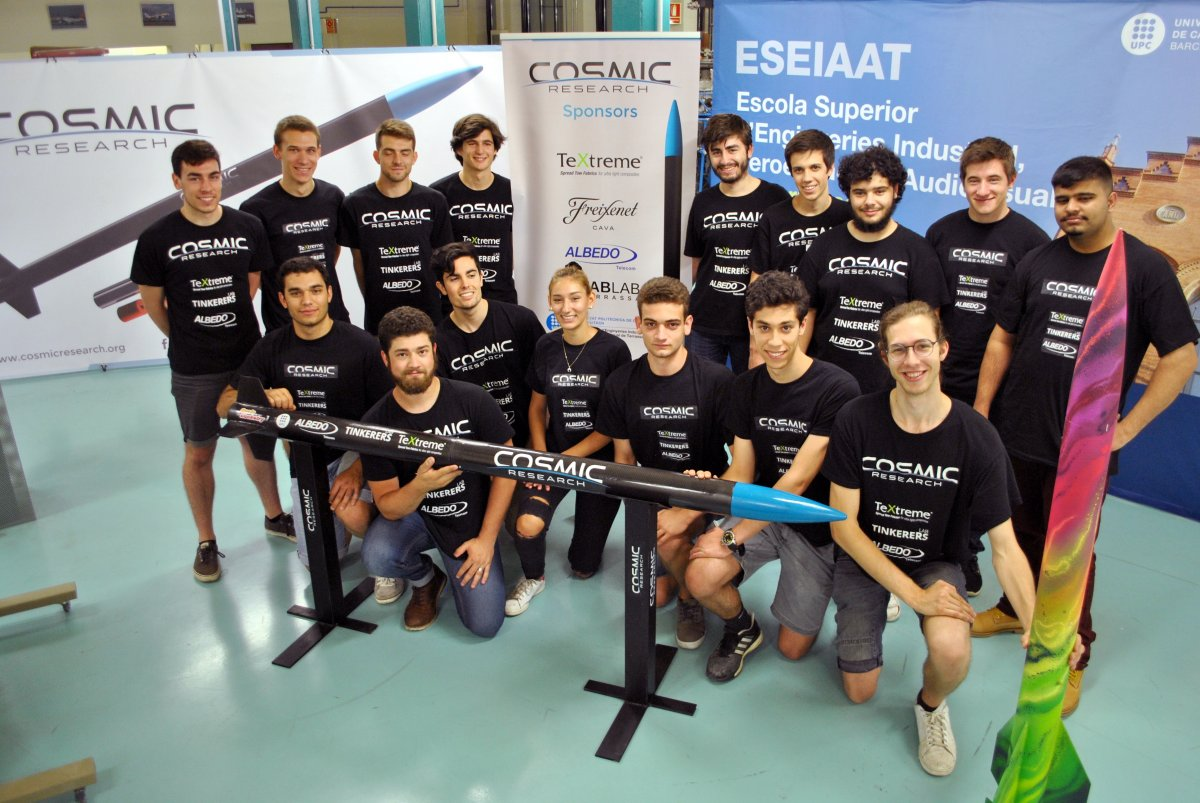
\includegraphics[width=250px]{images/cr.jpg}
    \end{frame}
    
    \begin{frame}
        \frametitle{Bondar (Sep 2017 - Q4 2018)}
        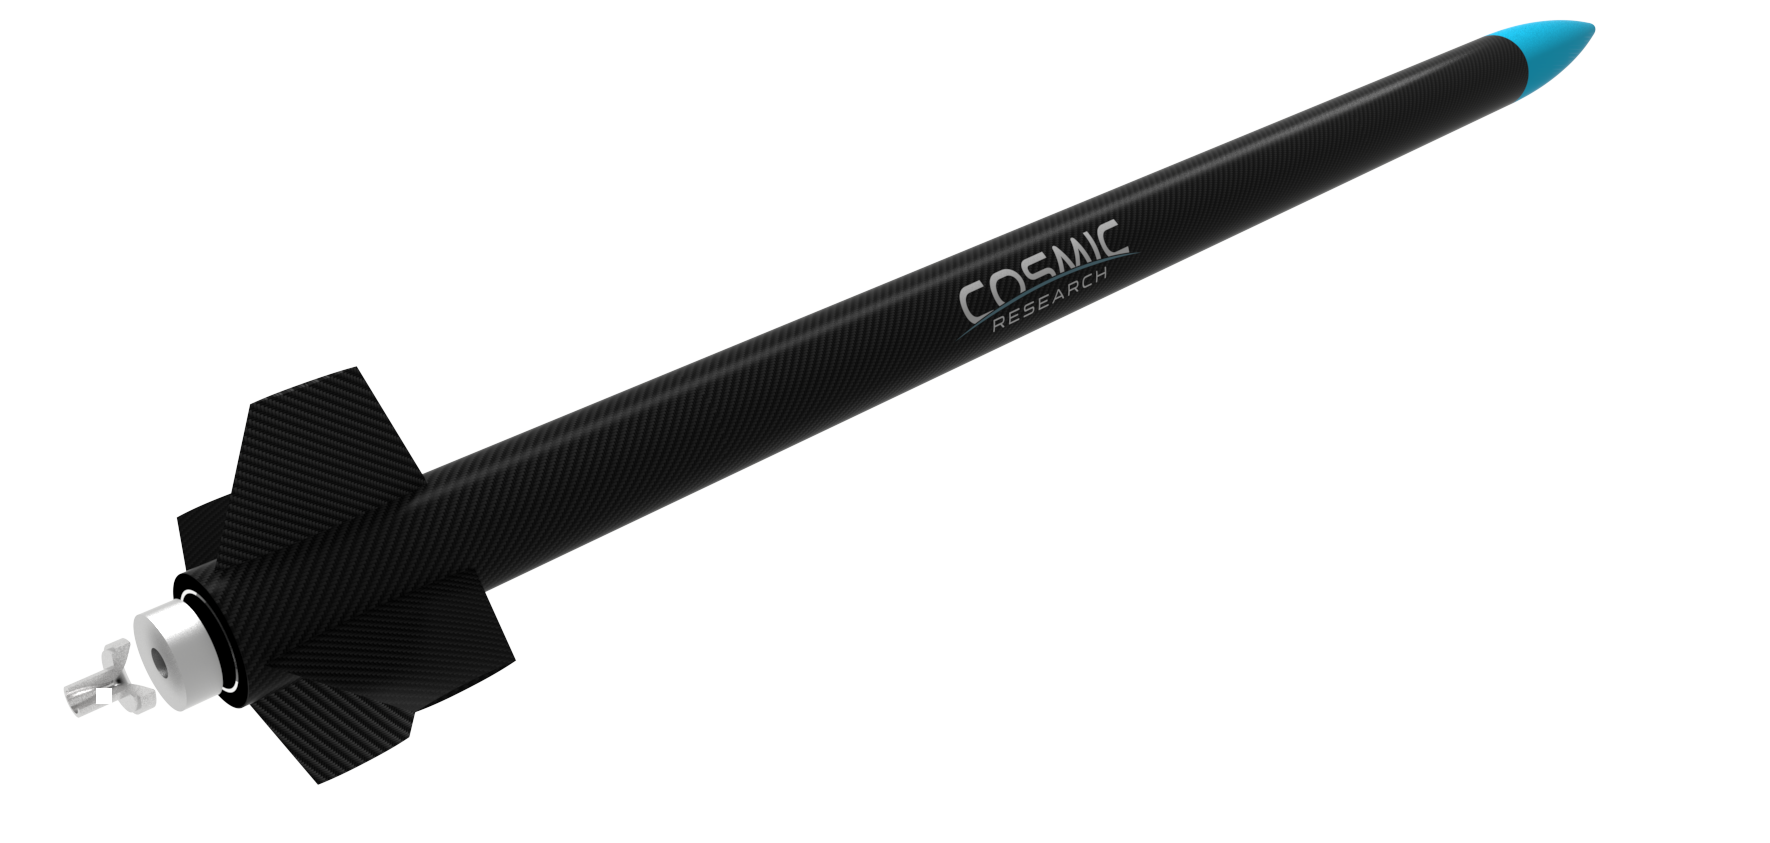
\includegraphics[width=\textwidth]{images/render.png}
    \end{frame}

    \begin{frame}
        \frametitle{Objectivos de la misión}
        \begin{enumerate}
            \item Desarrollar y probar las tecnologías que nos llevarán al espacio
            \item Alcanzar un apogeo máximo de 15-20km (alcanzar la estratosfera)
        \end{enumerate}
    \end{frame}

    \begin{frame}
        \frametitle{Aviónica}
        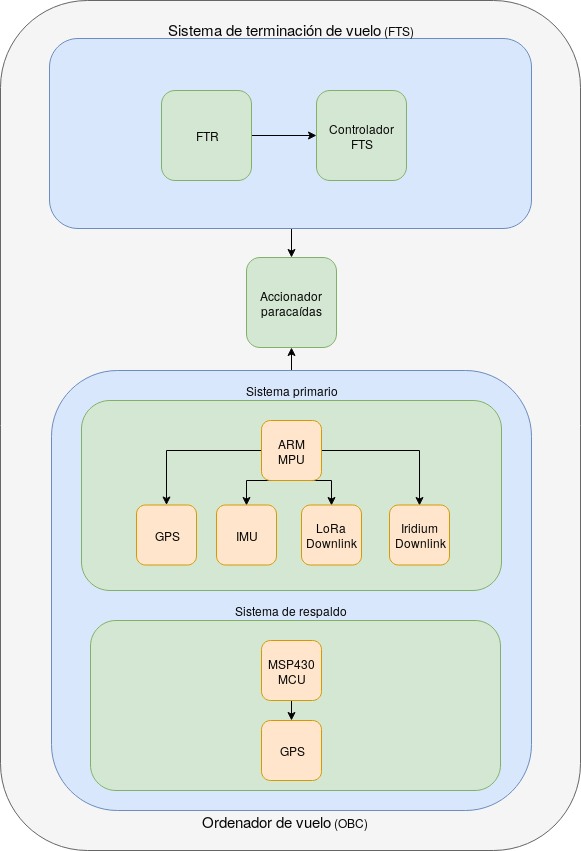
\includegraphics[height=0.8\textheight]{images/avionics.png}
    \end{frame}

    \begin{frame}
        \frametitle{Contribuciones}
        \begin{enumerate}
            \item \textit{Team Leader} del equipo de Aviónica
            \item Librería GPS
            \item \textit{Core} del firmware de la Aviónica
        \end{enumerate}
    \end{frame}
  
    \begin{frame}
        \frametitle{Librería GPS}
        \begin{itemize}
            \item Comunicación UART y procesado asíncronos
            \item (Re)Implementación de funciones de \textit{libc} como \textit{atof} o \textit{atoi}
            \item Procesado de sentencias NMEA 0183
        \end{itemize}
        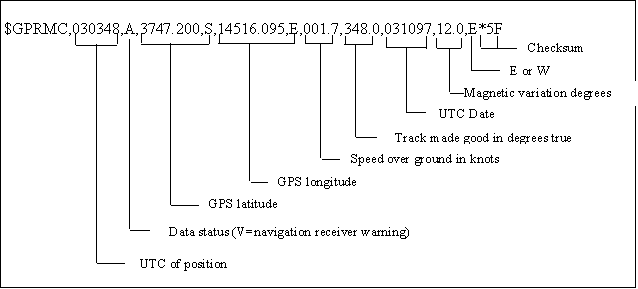
\includegraphics[width=\textwidth]{images/nmea.png}
    \end{frame}

    \begin{frame}
        \frametitle{\textit{Core} del firmware}
        \centering
        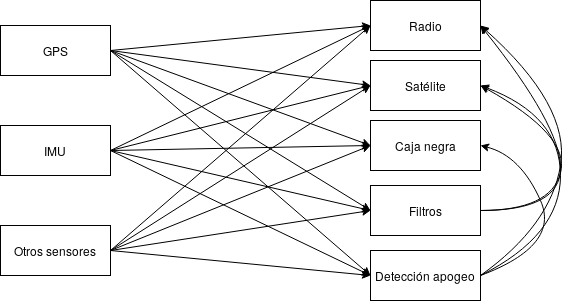
\includegraphics[width=0.9\textwidth]{images/problema.png}
    \end{frame}
    \begin{frame}
        \frametitle{Solución}
        \centering
        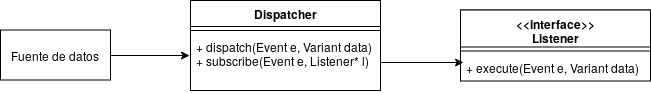
\includegraphics[width=0.9\textwidth]{images/solucion.png}
        \vfill
        Patrón Mediador-Observador orientado a Eventos
    \end{frame}
    \begin{frame}
        \frametitle{Problemas surgidos}
        \begin{enumerate}
            \item GCC abandonó el compilador después de lanzar la versión 4.6.3
            \item \textit{libc} limitada y con algunos bugs
            \item GCC solo soporta direccionamiento de 16 bits en una plataforma con direccionamiento de 20 bits
        \end{enumerate}
    \end{frame}
    \begin{frame}
        \frametitle{Perspectivas de futuro}
        \begin{enumerate}
            \item Actualmente estamos portando el firmware a ARM (Cortex-A5) con Linux
            \item El primer lanzamiento de pruebas está programado para Septiembre
            \item El lanzamiento final de la misión está programado para Q4 2018 - Q1 2019
        \end{enumerate}
    \end{frame}
    \begin{frame}
        \frametitle{Disponibilidad del software}
        \url{https://github.com/CosmicResearch/MSP430libs} \\
        \url{https://github.com/CosmicResearch/MSP430firmware} \\
        \url{https://github.com/CosmicResearch}
    \end{frame}
    \end{document}